\chapter{Overall Description}

\section{Product Perspective}
\subsection{Scnearios}
This section focuses on scenarios, which represent specific examples of interactions between
the system being developed and external actors in the environment. These scenarios are described
as concise narratives, intended to bridge the gap between system developers or designers and stakeholders,
who often lack technical expertise. Through detailed, tangible descriptions, scenarios provide a way for
developers to present straightforward examples of how the system might be used. This approach helps
stakeholders confirm their requirements and ensure alignment with their expectations. To achieve this,
the scenarios presented here are both creative and detailed, aiming to effectively convey the intended
concepts to the reader.
\subsubsection{SCENARIO 1 - Student logs in the system}
Marco is a university student at Politecnico di Milano, pursuing a degree in Computer Engineering.
The Politecnico di Milano has decided to rely on the Student\&Comapny platform to help its students
find an internship. 

Marco opens the S\&C website on his laptop and is greeted by a clean and intuitive login interface.
The platform prompts him to log in using his university credentials. He clicks on the "Login for Students"
button, which redirects him to his university’s authentication portal. Marco enters his student ID
and password, then confirms his identity.  

After successfully logging in, Marco is taken to his personalized dashboard. Here, he can immediately
see options to upload his CV, browse internship opportunities, and explore the system's features, such
as recommendations and feedback tools. Excited about the possibilities, Marco begins updating his
profile to enhance his chances of finding the perfect internship.
\subsubsection{SCENARIO 2 - Company logs in the system}
Elena is a recruitment manager at TechCorp, a mid-sized software development company specializing
in AI solutions. TechCorp has recently started offering internships to attract and nurture young talent,
and Elena wants to use the Students\&Companies (S\&C) platform to advertise their new openings.  

Elena opens the S\&C website on her office computer. The homepage greets her with a login interface.
Since TechCorp already has a registered account on the platform, Elena clicks on the "Login for
Companies" button. She is prompted to enter her company email and password. After filling in her
credentials and completing a two-factor authentication step, Elena successfully logs in.  

She is directed to TechCorp’s company dashboard. Here, she can view an overview of her active
internship postings, check pending student applications, and explore suggestions for refining
job descriptions to attract suitable candidates. Motivated to proceed, Elena decides to update one
of the internship postings and review the recommended student CVs tailored to TechCorp’s needs.  
\subsubsection{SCENARIO 3 - University logs in the system}
Laura is the internship coordinator at the University of Bologna, responsible for overseeing the
internships of students across various departments. The University of Bologna has decided
to rely on the Student\&Comapny platform to help its students find an internship.

Laura navigates to the S\&C platform website and is presented with the login interface.
She selects the "Login for Universities" option, which prompts her to enter her institutional
credentials. After typing in her university email and password, she successfully logs in and is
directed to the university-specific dashboard.  

On the dashboard, Laura can see a comprehensive overview of the internships involving students
from her university. She notices features to handle complaints, monitor internship statuses, and
view reports submitted by students and companies. Laura decides to review a recent complaint submitted
by a student and initiates the process to resolve the issue.
\subsubsection{SCENARIO 4 - Student modifies his/her profile and uploads his/her CV}
Giulia is a computer science student at the University of Florence and has recently
created an account on the Students\&Companies (S\&C) platform. After logging in, she decides to update her
profile to increase her chances of finding an internship that matches her skills and interests.  

From the dashboard, Giulia navigates to the "Profile Settings" section. Here, she updates
her personal information, including her current university program, areas of interest, and key
skills. She also adds details about her past experiences, such as a part-time job as a web developer
and a group project on machine learning completed during her studies.  

Next, Giulia clicks on the "Upload CV" button. She selects her CV file from her computer
and uploads it to the platform. Giulia saves her profile and returns to the dashboard, ready to
explore internship opportunities recommended by the platform.
\subsubsection{SCENARIO 5 - Company uploads its projects}
Marco, the project manager at InnovateTech, a leading tech firm specializing in artificial intelligence
solutions, is responsible for managing the company’s internship program. To attract the right candidates,
he decides to upload the company’s projects to the Students\&Companies (S\&C) platform.  

He logs into the platform using his company credentials. From the company dashboard, he navigates to
the "Project Management" section. Here, Marco clicks on the "Upload New Project" button. He is prompted
to fill out a form detailing the project title, description, tasks, and required skills. Marco provides
a detailed description of the project, including the application domain, the technologies used, and the
learning outcomes for interns. He also specifies the terms of the internship, such as whether it is paid,
and if there are any additional benefits like training or mentorship.  

After reviewing all the details, Marco uploads the project to the platform. The project is now available
for students to view when they search for internships that match their skills and interests. Marco feels
confident that this will help attract suitable candidates to InnovateTech’s internship program.
\subsubsection{SCENARIO 6 - Student receives recommendations regarding projects that may be of interest to him}
Alessandro, a computer science student at the University of Naples, has been actively using the
Students\&Companies (S\&C) platform to explore internship opportunities. One day, he receives a
notification from the platform highlighting projects that align with his skills and interests.

Alessandro logs into his account and finds a list of recommended projects tailored to his profile.
Each project listing provides a brief description, the required skills, and the terms offered by
the companies. He can easily review these details or express interest in projects he likes.
This feature helps Alessandro stay informed about new opportunities and makes it easier for
him to connect with companies offering internships that match his goals.
\subsubsection{SCENARIO 7 - Company receives recommendations regarding students who might be interesting for its projects}
Marco, the project manager at InnovateTech, logs into the Students\&Companies (S\&C) platform
to check on potential candidates for the company’s internships. He receives a notification
from the platform suggesting students whose profiles match the requirements of InnovateTech’s projects.
These recommendations are based on the students’ skills, experiences, and interests, as well as
the project details Marco previously uploaded.

He can review the students’ CVs, see their academic
backgrounds, and assess their fit for the roles available. This feature helps Marco quickly identify
 promising candidates and streamline the hiring process for InnovateTech’s internship program.
\subsubsection{SCENARIO 8 - Student applies for a position and starts the selection process}
Maria, a computer science student at Politecnico di Milano, is exploring internship opportunities
on the Students\&Companies (S\&C) platform. She finds a project that aligns with her skills and
interests and decides to apply. Maria clicks the "Apply" button on the project page, expressing
her interest in the position. S\&C promptly notifies the company about her request.

The compan then reviews Maria’s profile, considering her academic background and relevant
experiences listed on her CV. If they find her a good fit for the project, the company accepts
her into the selection process.
\subsubsection{SCENARIO 9 - Company manages the student's selection process}
John, the HR manager at TechInnovators, logs into the Students\&Companies (S\&C) platform
to manage the selection process for an internship position. He clicks the button to allow a student,
Maria, to fill out the preliminary questionnaire. S\&C promptly notifies Maria that she can start
the questionnaire. Maria completes the questionnaire, providing her background, skills, and experiences.
S\&C then notifies John that Maria has filled out the questionnaire. In the platform’s dedicated
private space, John reviews Maria’s responses and assesses her suitability for the role.

Next, John invites Maria to an online interview. S\&C sends Maria a notification containing the
date and time of the interview. A reminder notification is sent to Maria at the scheduled time
of the appointment, ensuring she doesn’t miss it. During the interview, John evaluates Maria’s fit
for the position, asking questions and discussing her experiences and goals. After the interview,
John updates the platform with his notes and assessment of Maria’s performance. The platform helps
John keep track of Maria’s progress throughout the selection process.

Once Maria is selected for the internship, S\&C automatically sends her a notification informing her
of the decision. This notification ensures that Maria is kept in the loop about her selection status
without needing to log in to the platform regularly. John finalizes the selection of Maria directly
on the S\&C platform, and Maria receives a final confirmation notification about her acceptance into
the internship program.
\subsubsection{SCENARIO 10 - Company manages the student's internship}
John, the HR manager at TechInnovators, has finalized the selection of Maria for an internship position.
Once the selection is confirmed, S\&C creates a dedicated page for Maria’s specific internship, where
all official announcements and updates will be posted. S\&C then opens a communication channel between
John and Maria. Both John and Maria receive notifications informing them that the communication channel
is now open. John begins by writing important information about the start of Maria’s internship in the
dedicated space. S\&C notifies Maria about the publication of this information, ensuring she is
well-informed about the internship’s details.

From that moment, Maria and John can communicate through the platform using the communication channel,
following scenario 11 for communication. This allows John to provide regular updates,
answer Maria’s questions, and keep her informed about her responsibilities and ongoing projects.
John also uses the dedicated space to post information about the current status of the internship,
such as task updates or project milestones. Maria responds by writing comments in the dedicated space,
engaging actively in the ongoing discussions.

As approaches the end of her internship period, John confirms the end of the internship through
the dedicated space. S\&C then notifies Maria and John that the internship is over. The communication
channel is then closed, and the dedicated page for Maria’s internship is deleted by S\&C. This ensures a smooth and organized closure
to Maria’s internship, leaving both Maria and John well-prepared for future opportunities.
\subsubsection{SCENARIO 11 - Student and company communicate with each other}
Maria, a computer science student at the Politecnico di Milano, has just started her internship at
TechInnovators. To ensure smooth communication throughout the internship, S\&C provides a dedicated
communication channel between Maria and John, the HR manager overseeing her internship.  

At the beginning of the internship, John uses the communication channel to send Maria important
information about her first tasks and upcoming deadlines. Maria promptly replies, confirming
she has received the details and asking clarifying questions about specific requirements.
The clear and structured communication ensures Maria knows exactly what is expected of her.  

A few weeks into the internship, Maria encounters a challenge while working on her assigned project.
She uses the communication channel to notify John about the issue, explaining the technical difficulty
and proposing potential solutions. John reviews her message and quickly responds with guidance,
offering support from the IT department if needed.  

During the internship, John also uses the channel to address minor concerns regarding
Maria’s punctuality in submitting weekly updates. He communicates this issue politely,
asking if there are any difficulties impacting her workflow. Maria appreciates the constructive
feedback and commits to improving her timeliness.  

Similarly, Maria uses the channel to provide her feedback on the internship experience.
She notes that the initial onboarding process was slightly overwhelming and suggests a more
gradual introduction to company tools for future interns. John thanks Maria for her input and
assures her that her suggestions will be taken into consideration for improvement.  

Toward the end of the internship, both Maria and John use the channel to coordinate the final
tasks and confirm the submission of her final project. The communication remains professional
and efficient, with both parties ensuring that all expectations are met before the internship
concludes.  

The S\&C communication channel proves invaluable in maintaining open, transparent, and respectful
interactions between Maria and John. It helps manage tasks, resolve issues, and address concerns,
ensuring a positive and productive internship experience for both parties.
\subsubsection{SCENARIO 12 - Student responds to the feedback requested by the system}
Maria, a computer science student from Politecnico di Milano, is participating in an internship
at TechInnovators, secured through the S\&C platform. During both the selection process and the
internship, S\&C periodically requests feedback from students like Maria to ensure a high-quality
experience.  

While still in the selection process, Maria received a notification prompting her to answer questions
about her experience. She was asked about the clarity of communication with the company, the usefulness
of the interview preparation, and her overall satisfaction so far. Maria quickly provided her input,
appreciating the platform’s proactive approach.  

Later, during the internship, Maria received another notification asking her to evaluate her
current experience. She shared feedback about her assigned tasks, the mentorship provided,
and the work environment, noting both positive aspects and areas for improvement.  

Maria felt valued throughout the process, knowing her feedback was contributing to improving
internships for herself and future participants.
\subsubsection{SCENARIO 13 - Company responds to the feedback requested by the system}
TechInnovators, a dynamic software development company, started using the S\&C platform
to find talented students for their internships and has recently selected for an internship Maria,
a computer science student from Politecnico di Milano. John, the manager supervising Maria,
finds the system helpful not only for selecting candidates but also for maintaining a structured
internship process.  

During the selection phase, the S\&C platform sent a notification to John, asking for feedback
on how effectively the system matched candidates with the project requirements. The questions
included topics like the clarity of student profiles, the quality of the preliminary questionnaires,
and the interview process. John completed the form, noting that Maria’s profile was well-aligned with
the company’s needs, and he appreciated the platform’s intuitive design.  

Halfway through the internship, the system sent another feedback request. This time, the focus
was on Maria’s performance and the internship experience. John received a notification and took
a few minutes to answer questions about her progress, technical skills, and her integration within
the team. He commended Maria for her proactivity and ability to learn quickly, while also suggesting
minor adjustments to the S\&C platform to provide companies with additional onboarding resources.  

The feedback process helped TechInnovators evaluate their own practices and ensure a productive
internship experience, while S\&C ensured the feedback loop was seamless and efficient.
\subsubsection{SCENARIO 14 - University receives the complaint report}
At the Politecnico di Milano, Professor Marco Bianchi, responsible for overseeing internships
in the Computer Engineering department, receives a notification from the S\&C platform.
The notification informs him that a complaints report related to ongoing internships has
been prepared and is ready for review.  

Marco logs into the platform and navigates to the "Complaints" section. There, he finds
a detailed report outlining issues raised by students and companies. One of the complaints
is from Luca, a computer engineering student interning at Innovatech, who reported insufficient
guidance during the development of a software module he was assigned. Another complaint comes
from Clara, the HR manager at Innovatech, who flagged delays in Luca’s completion of his weekly
progress updates.  

S\&C’s organized format allows Marco to quickly assess the situation, with each complaint
categorized and accompanied by relevant timestamps. Recognizing the importance of resolving
these issues promptly, Marco decides to reach out to both Luca and Clara to discuss the concerns
and find a resolution that benefits both parties.  

Thanks to S\&C’s efficient reporting and notification system, Marco can act swiftly to
maintain the quality and integrity of the internship experience.
\subsubsection{SCENARIO 15 - University interrupts internship}
Luca, a computer engineering student at the Politecnico di Milano, has been facing significant
issues during his internship at Innovatech. Professor Marco Bianchi, responsible for managing
internships, has received multiple complaints from both Luca and Clara, the HR manager at Innovatech.
These complaints indicate serious concerns regarding Luca's guidance and communication throughout
the internship.  

Upon reviewing the complaints and the ongoing situation, Professor Bianchi decides to visit the
"Internship Interruption" page on the S\&C platform. Here, he selects Luca as the student in
question and then picks the Innovatech internship. 

Marco then clicks the button to interrupt the internship. Once confirmed, S\&C promptly notifies
both Luca and Clara about the decision. For Luca, the notification explains that his internship
with Innovatech has been officially interrupted due to unresolved issues. For Clara, the
notification informs her that Luca will no longer be interning at Innovatech.  

This process ensures clear communication and quick action, maintaining the integrity of
the internship program at Politecnico di Milano.
\newpage
\subsection{Domain Class Diagram}
The class diagram provided below offers a high-level overview of the domains of interest
for the software implementation.
The diagram can be divided into three main sections:

The central section contains the main entities related to users: Student, student profile,
company, proposed interview, and university.

The lower section illustrates the primary interactions between students and companies necessary
for successfully performing an internship: Preliminary match, selection process, final match,
and internship. This area also includes important management classes such as SelectionProcessManager
and InternshipManager.

The upper section displays the main classes related to the recommendation system.
It includes classes for feedback and preliminary data collection, which are then sent
to the analysis system to generate recommendations (also represented by a class).
Finally, this system sends notifications, represented by another class, which connects
to the user superclass.

\begin{figure} [H]
    \centering
    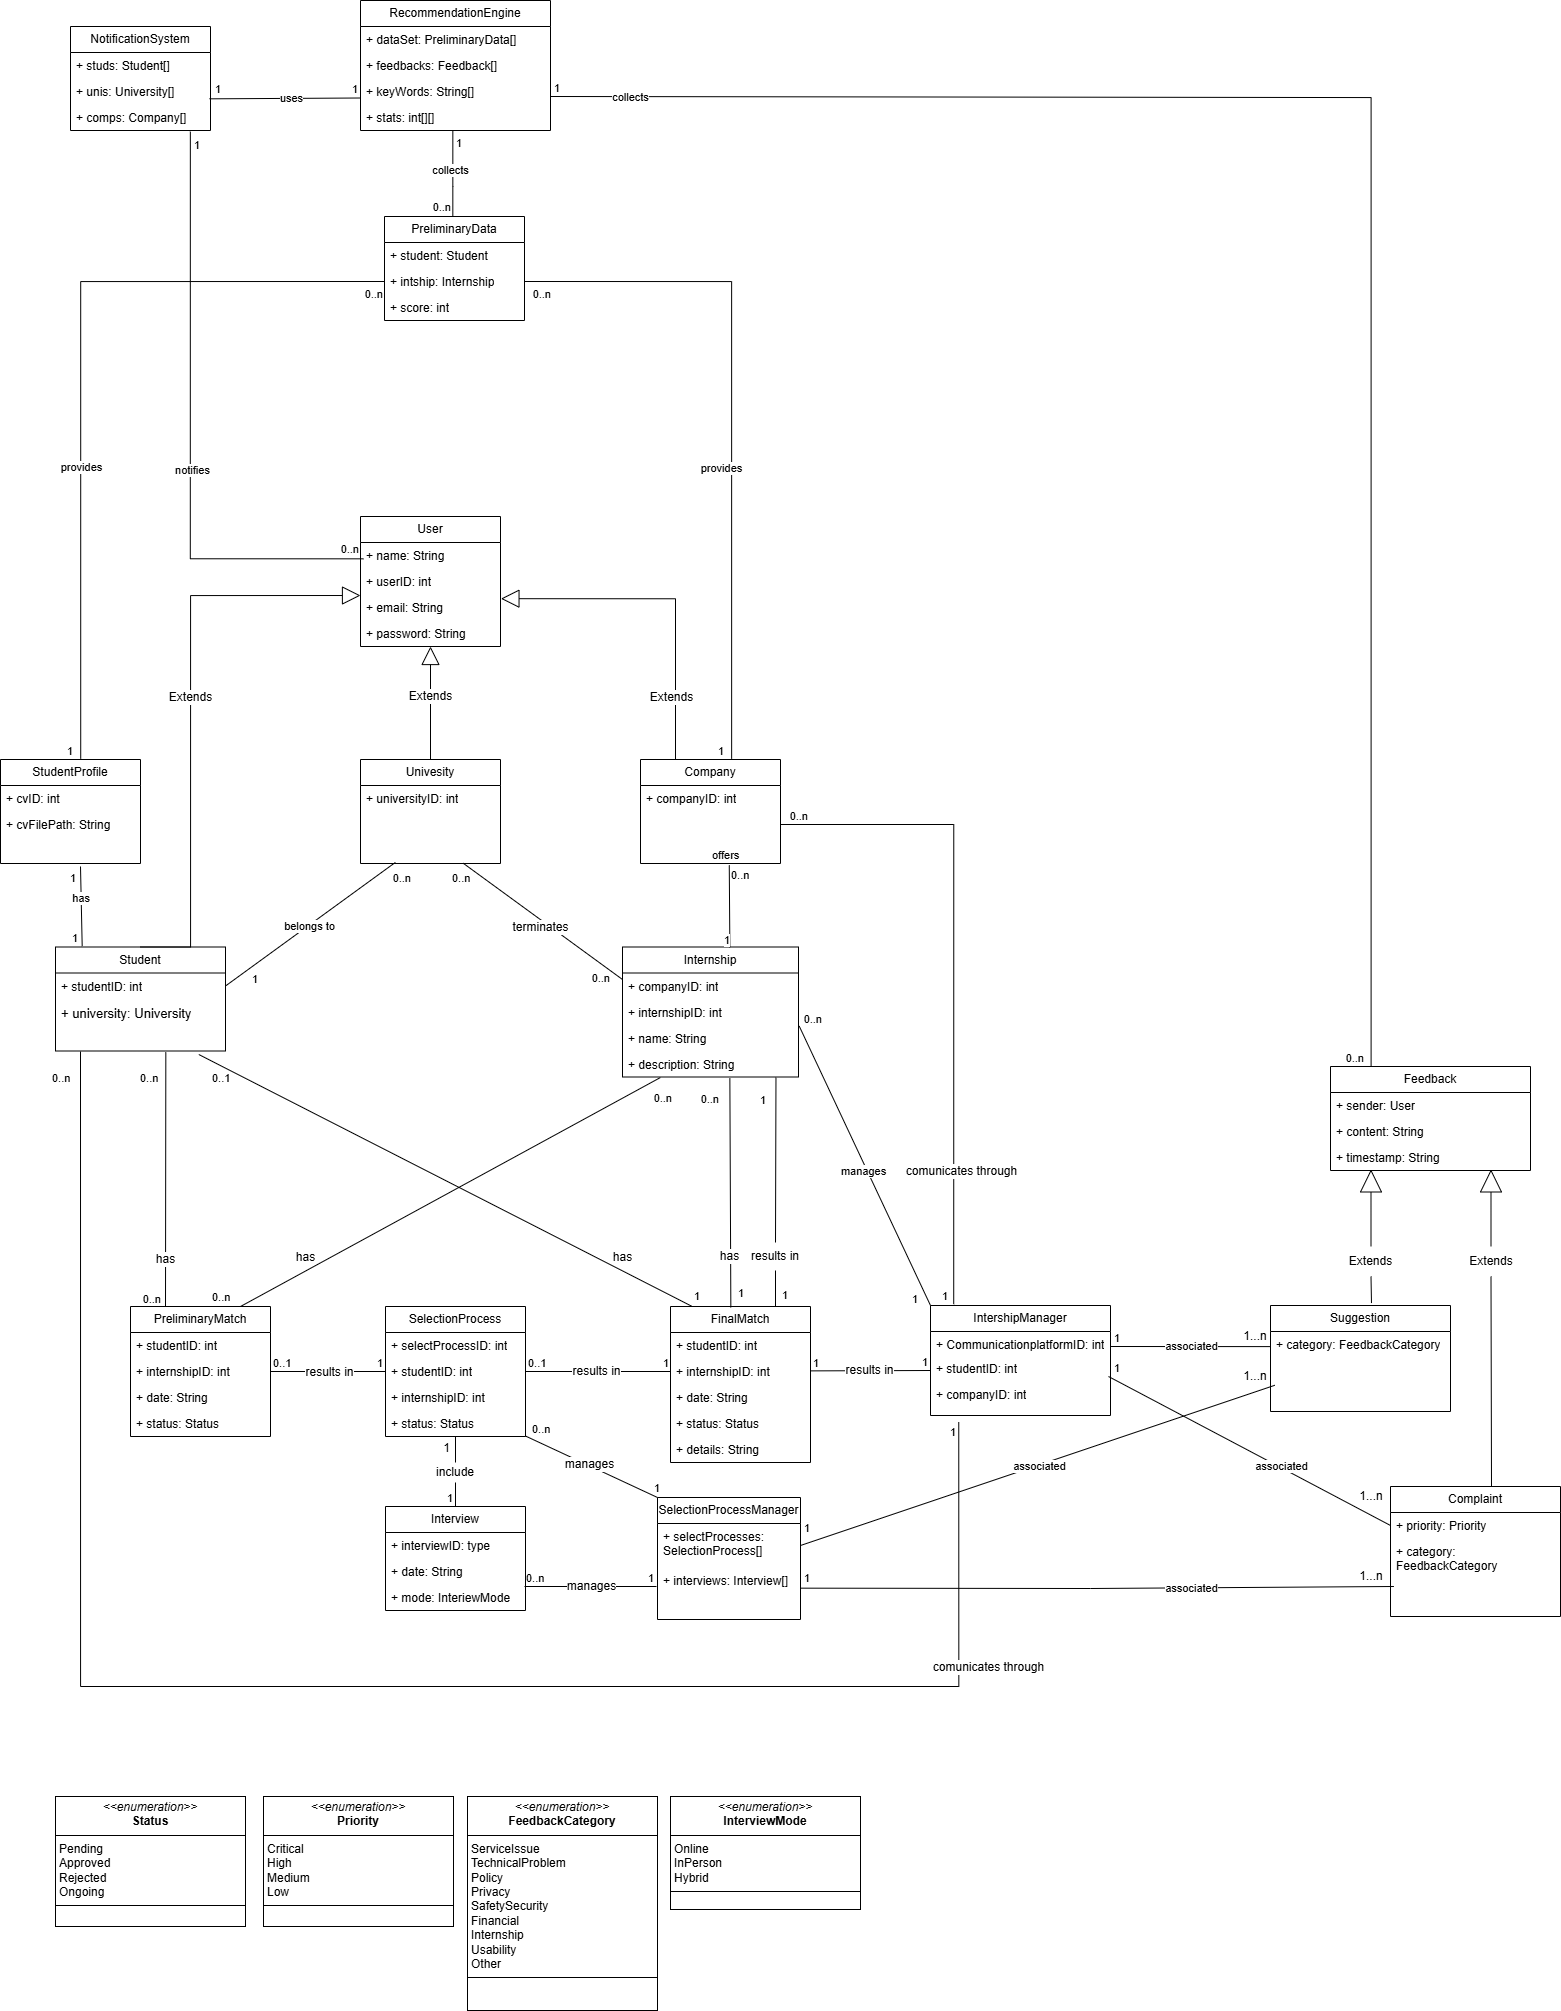
\includegraphics [width=1\linewidth] {ClassDiagram.png}
    \caption{Class Diagram}
\end{figure}

\newpage
\subsection{State Charts}
In this section, we analyze the state charts related to the selection process and the management
of complaints by universities. We believe these two scenarios are the most significant to represent
with this type of diagram due to their structured sequences of well-defined events.

\subsubsection{Selection Process}


\begin{figure} [H]
    \centering
    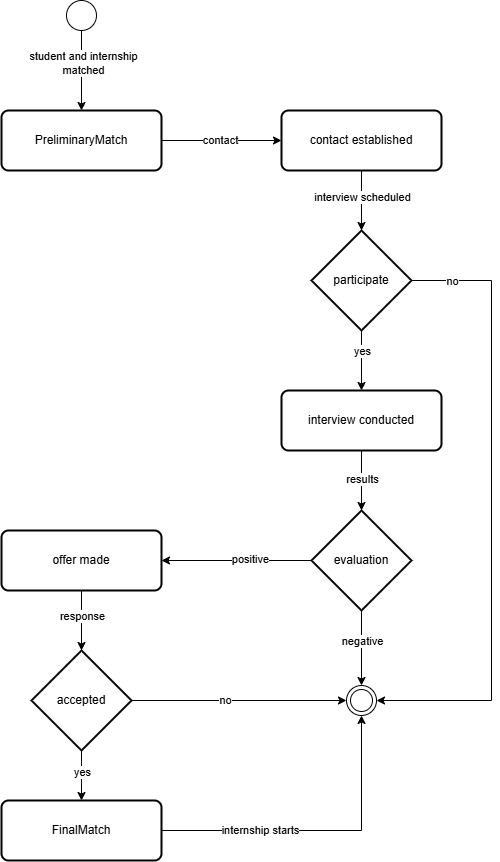
\includegraphics [width=.4\linewidth] {sc_SelectionProcess.png}
    \caption{State Charts 1 - Selection Process}
\end{figure}

The diagram illustrates the phases of the selection process. The initial stage begins
with the student being matched to an internship opportunity,
represented as the "PreliminaryMatch" state. Once the match occurs, the intermediary
system, referred to as S\&C, establishes contact between the company and the student,
transitioning the process to the "contact established" state.

At this point, an interview is scheduled. If the student does not participate in the
interview, the process halts. However,
if the student participates, the interview is conducted, leading to the evaluation phase.

During the evaluation, the company assesses the student’s performance and suitability.
If the evaluation is positive, the company makes an offer, indicated as the "offer made" state.
If the evaluation is negative, the process terminates without any further steps.

Following the offer, the next stage depends on the student’s response. If the student
declines the offer, the process concludes without an agreement. On the other hand,
if the student accepts, the process progresses to the "FinalMatch" state. At this point,
the internship officially begins, marking the finalization of the selection process.

\subsubsection{Complaints management}


\begin{figure} [H]
    \centering
    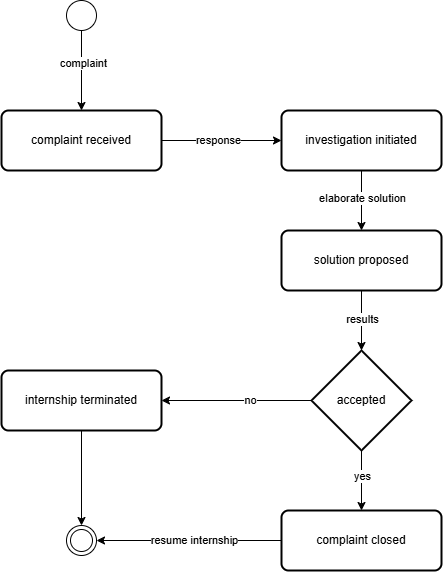
\includegraphics [width=.4\linewidth] {sc_UniComplaint.png}
    \caption{State Charts 2 - Complaints management}
\end{figure}

The diagram illustrates the complaint management process within the context of an internship.
The flow begins when a complaint is received, prompting an investigation to examine the issue.
Once the investigation is completed, a solution is proposed to address the complaint.
At this stage, a critical decision determines the outcome.

If the proposed solution is accepted, the complaint is closed, and the internship can
continue as usual. However, if the solution is not accepted, the internship is terminated,
bringing the process to an end.

This diagram clearly highlights the two possible outcomes of the complaint resolution process:
a positive resolution, which results in the complaint being closed, or a negative outcome,
which leads to the termination of the internship.



\newpage
\section{Product Functions}
\subsection{Requirements}
This section presents a detailed list of functional requirements that Student\&Comapny
must fulfill during its development. Functional requirements define the operations
and decisions the system under consideration must perform to satisfy the needs of
its stakeholders. These requirements have been derived through a process of elicitation
and abstraction, as discussed in the earlier sections of this document.
The analysis of relevant aspects within the domain, the validation of stakeholder
needs through scenarios, and the visual representations offered by various diagrams provide
a strong foundation for the design phase outlined in the subsequent part of this document.

\subsubsection{G1 - The system allows students to proactively look for internships}
\hspace*{15mm}
\begin{itemize}
    \item [R 1.1] - The system allows students to create their profile.
    \item [R 1.2] - The system allows students to upload their CV.
    \item [R 1.3] - The system provides suggestions to students on how to submit their CV.
    \item [R 1.4] - The system allows students to browse internships.
\end{itemize}
\hspace*{15mm}

\subsubsection{G2 - The system allows companies to advertise the internships that they offer}
\hspace*{15mm}
\begin{itemize}
    \item [R 2.1] - The system allows companies to create their profile.
    \item [R 2.2] - The system allows companies to upload their internships.
    \item [R 2.3] - The system provides suggestions to companies on how to submit their internship descriptions.
\end{itemize}
\hspace*{15mm}

\subsubsection{G3 - The system recommends students about suitable internships and recommends
companies about student CVs corresponding to their needs}
\hspace*{15mm}
\begin{itemize}
    \item [R 3.1] - The system notifies students about suitable internships.
    \item [R 3.2] - The system notifies companies about suitable student CVs.
    \item [R 3.3] - The system recommends based on keyword searching.
    \item [R 3.4] - The system recommends based on the characteristics of students and internships.
    \item [R 3.5] - The system recommends based on statistical analysis.
    \item [R 3.6] - The system collects information regarding the internship.
    \item [R 3.7] - The system asks students and companies to provide feedback and suggestions.
\end{itemize}
\hspace*{15mm}

\subsubsection{G4 - The system allows students and companies to stipulate a mutual contract
which establishes the start of the selection process and its management}
\hspace*{15mm}
\begin{itemize}
    \item [R 4.1] - The system allows students to apply for an internship.
    \item [R 4.2] - The system allows companies to accept student applications.
    \item [R 4.3] - The system allows students to sign the contract for the internship.
    \item [R 4.4] - The system allows companies to sign the contract for the internship.
    \item [R 4.5] - The system supports the selection process by helping manage interviews and also finalise the selections.
\end{itemize}
\hspace*{15mm}

\subsubsection{G5 - The system allows internship's management and communication between the two parties
throughout the ongoing internship process}
\hspace*{15mm}
\begin{itemize}
    \item [R 5.1] - The system provides spaces for the official announcements.
    \item [R 5.2] - The system provides spaces where interested parties can complain,
    communicate problems, and provide information about the current status of the ongoing internship.
\end{itemize}
\hspace*{15mm}

\subsubsection{G6 - The system allows universities to monitor the situation and handle complaints.}
\hspace*{15mm}
\begin{itemize}
    \item [R 6.1] - The system allows universities to create their profile.
    \item [R 6.2] - The system allows universities to monitor the situation of internships and handle complaints.
    \item [R 6.3] - The system allows universities to interrupt an internship.
\end{itemize}
\hspace*{15mm}


\section{User Characteristics}
\subsection{Student}
\subsection{Company}
\subsection{University}

\section{Assumptions, Dependencies and Constraints}
\subsection{Domain Assumptions}